\section{Motivation}

One of the main objectives in computer vision is that of recognising instances of an object category (e.g. cars, pedestrians, faces,...) in images or videos. This has many useful applications like cameras that automatically bring faces into focus, video surveillance systems that track certain objects, traffic monitoring, and roboter vision to name just a few. When given an image the goal of a typical object detection system is to list whether one or several instances of a pre-trained object class are present, and to indicate its position in the image via a rectangular bounding box, tightly covering the object instance (see figure \ref{fig:vocEx}).
\begin{figure}
\begin{center}
        \begin{subfigure}[b]{0.49\textwidth}
                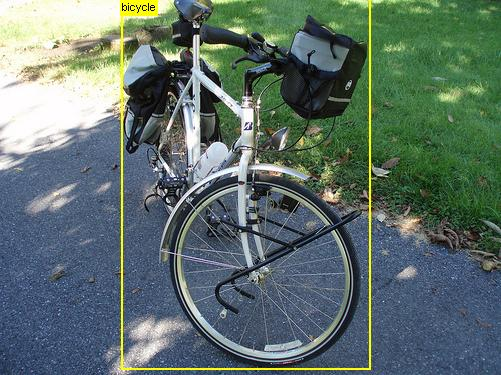
\includegraphics[width=\textwidth]{vocEx1}
        \end{subfigure}
        \begin{subfigure}[b]{0.49\textwidth}
               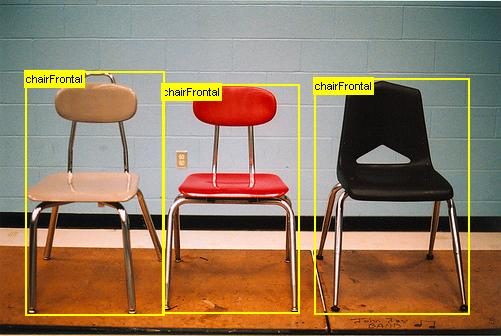
\includegraphics[width=\textwidth]{vocEx2}
        \end{subfigure}
\caption{Examples from the Pascal Visual Object Classes (VOC) challenge 2012. \cite{pascal-voc-2012}}
\label{fig:vocEx}
\end{center}
\end{figure}

Object category recognition remains one of the most challenging goals of computer vision. While for us humans it is mostly a trivial and effortless task, teaching a computer to recognise objects is very challenging. Given an image, all the computer initially "sees" are numbers referring to the RGB values of each image pixel. Today, the arguably most important step towards teaching machines how to see is to translate these pixel values into more meaningful and task-suited representations (features) of  an image. 

An object recognition system has to deal with a lot of variation between object classes (inter-class variability) as well as inside of object classes (intra-class variability). Cats for example are very different from cars in that they are non-rigid, have a furry texture, etc. and the system should be able to identify and discriminate between both. A recognition system for cars has to be able to detect cars of all sorts of different sizes and types and should also be able to recognise them from any viewpoint. 

One of the most widely used and successful approaches to object recognition in the last decade was the Deformable Parts Model (DPM) \cite{5255236}. It combines effective scale-invariant Histograms of Oriented Gradients (HOG) features \cite{1467360} with a deformable geometric model and mixture models that allow it to model intra-class variation effectively for many object classes. Current state of the art results in object detection are achieved by systems based on Convolutional Neural Networks (CNN) \cite{girshick2013rich}, a technique that made an impressive comeback thanks to the possibilities of GPU-programming (which made efficient training possible) and the existence of large datasets \cite{krizhevsky2012imagenet}.

\begin{figure}
\begin{center}
        \begin{subfigure}[b]{0.43\textwidth}
                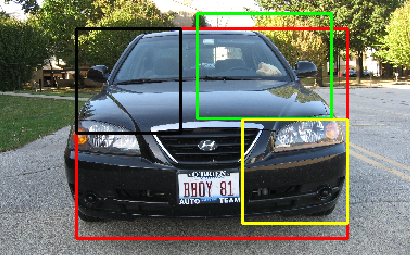
\includegraphics[width=\textwidth]{view1}
        \end{subfigure}
        \begin{subfigure}[b]{0.43\textwidth}
               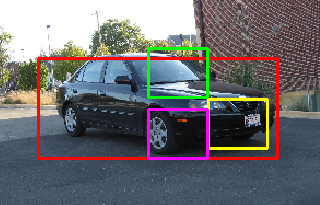
\includegraphics[width=\textwidth]{view2}
        \end{subfigure}
        \begin{subfigure}[b]{0.43\textwidth}
                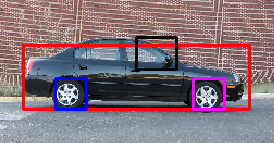
\includegraphics[width=\textwidth]{view3}
        \end{subfigure}
        \begin{subfigure}[b]{0.43\textwidth}
               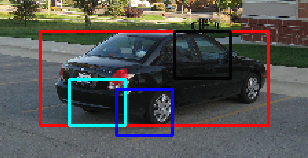
\includegraphics[width=\textwidth]{view4}
        \end{subfigure}
        \begin{subfigure}[b]{0.43\textwidth}
                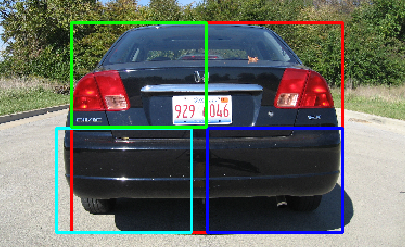
\includegraphics[width=\textwidth]{view5}
        \end{subfigure}
        \begin{subfigure}[b]{0.43\textwidth}
               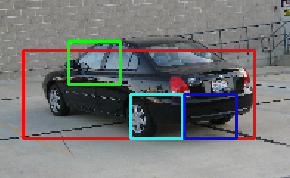
\includegraphics[width=\textwidth]{view6}
        \end{subfigure}
        \begin{subfigure}[b]{0.43\textwidth}
                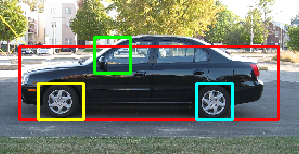
\includegraphics[width=\textwidth]{view7}
        \end{subfigure}
        \begin{subfigure}[b]{0.43\textwidth}
               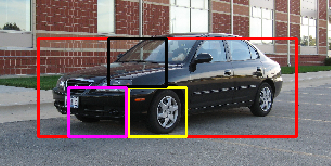
\includegraphics[width=\textwidth]{view8}
        \end{subfigure}                
\caption{This figure shows detections of an eight-viewpoint-3D-DPM with six 3D-parts and three parts per viewpoint. The red boxes indicate the root filter placement and the other boxes indicate part placements. Each 3D part is assigned a separate  colour to help illustrate their consistent 3D placement. Note that this model was trained with a small number of parts for illustration purposes. The images are taken from the 3D Objects Dataset of \cite{4408987}.}
\label{fig:carviews}
\end{center}
\end{figure}

Very often, more information than just the presence and location of an object would be useful. To arrive at a better scene understanding, we might, for example, like to know the viewpoint that an image of an object was taken under. For this reason, there was a recent growth of interest for 3D object representations. The arguably most successful 3D models today are based on the DPM and have delivered impressive results in viewpoint recognition while upholding and in some cases even increasing 2D bounding box localisation \cite{6248075,Pepik:2012aa}. The extension of a DPM to 3D is usually done by anchoring object parts in three-dimensional space and modelling a discrete number of viewpoints. Modelling objects under a set of discrete viewpoints requires to have viewpoint information provided in the training data and introduces additional supervision to the training procedure. It is interesting to note however that a normal 2D DPM very often learns objects under specific viewpoints, therefore justifying the approach of the 3D model. The mapping of the 3D part position to the 2D image plane during test-time is done via a viewpoint dependant projective mapping. Part appearances are learned for each model viewpoint separately, with the constraint that they have to be consistent across views. This is important as otherwise the 3D information of the model reduces to basically just a number of different object views. Figure \ref{fig:carviews} illustrates the consistent 3D learning of part appearances on detections of the 3D-DPM implemented in this project. Detections for the same car are shown for eight viewpoints that the model was trained on. In contrast to detections of a usual 2D-DPM (see figure \ref{fig:dpmcar}), which models parts independently for different views, we observe that the parts detected with the 3D-DPM have a 3D geometric relationship. To enforce the 3D constraints on the model, exact viewpoint information for several views of the same object instance are needed. This information is usually provided by  renderings of Computer Aided Design (CAD) models. 


\begin{figure}
\begin{center}
        \begin{subfigure}[b]{0.49\textwidth}
                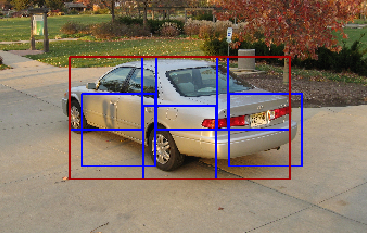
\includegraphics[width=\textwidth]{dpmcar1}
        \end{subfigure}
        \begin{subfigure}[b]{0.49\textwidth}
               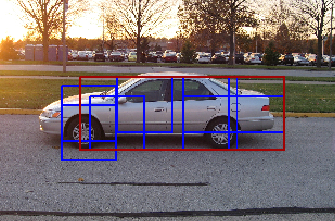
\includegraphics[width=\textwidth]{dpmcar2}
        \end{subfigure}              
\caption{This figure shows detections of a normal 2D-DPM. The red boxes indicate the root filter placement and the blue boxes indicate part placements. Note that there is no apparent connection between parts of the two different views.}
\label{fig:dpmcar}
\end{center}
\end{figure}

The aim of this project is to implement and study a 3D deformable parts model for the detection and pose-estimation of cars. The implementation will be based on the successful and openly available implementation of the original DPM \cite{5255236}. The study will cover the use of new annotated training data, implementation details, an evaluation of model and training parameter choices, experiments on well known and challenging datasets and a comparison to other models. Furthermore, it will also cover the incorporation of features obtained from Convolutional Neural Networks into the model and how these affect the training procedure and the performance of a 3D-DPM. 


\section{Outline}

This thesis is structured into  three main chapters. Chapter \ref{chap:back} provides an overview of the research field at hand and gives a review of related work. Also, a brief introduction to the two image-descriptors (features) used in the project will be given. This chapter sets the context for the research in this thesis.

In chapter \ref{chap:model}, the model implemented in this project will be introduced. In section \ref{sec:dpmreview} a review of the original DPM (on which it is based on) will be  provided and a formal framework for the model will be set up. Section \ref{sec:ext3D} will then explain the modifications made to the DPM to arrive at a 3D object model. Finally, section \ref{sec:cnnFeat} explains the steps taken to replace the HOG features of the original DPM with features obtained from Convolutional Neural Networks.

Chapter \ref{chap:exp} shows and discusses experimental results obtained on several datasets and puts them into context with other work. It also discusses the influence of several model parameters on the model's performance on bounding box localisation and viewpoint estimation.

Finally, chapter \ref{chap:conclusion} will conclude the thesis by providing a review of the results and insights gained throughout the project. It will also discuss ideas for future research work building on this thesis.
